\section{Cube Moves keep}

Each move of the \rubik{} will be described by using a slightly modified cycle notation. A description of what happens to each oriented cubie will be needed, so it will describe where each cubie moves and where each face of the cubie moves. For example, if the \rubik{} is unfolded, then draw the down face, so it will look like the following:


\begin{figure}[h]
	\centering	
		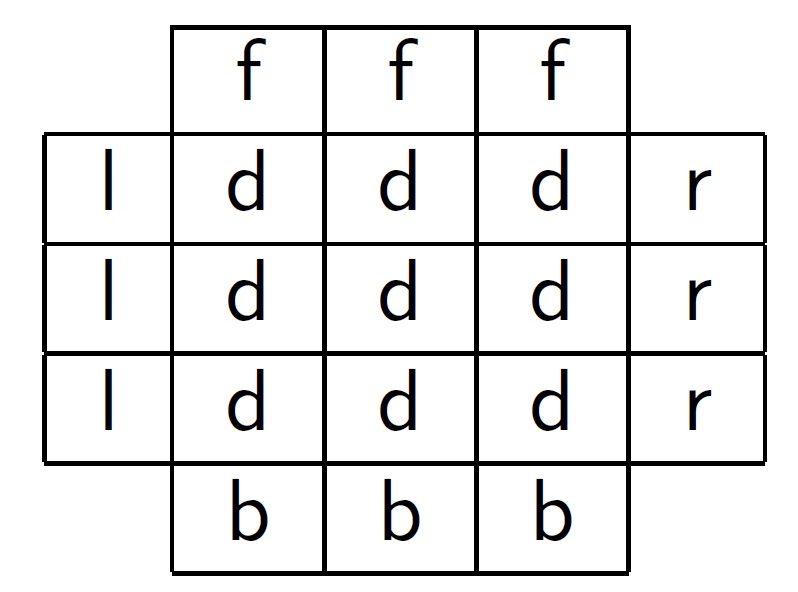
\includegraphics [scale=0.2]{input/pics/rubiks1.jpg}
			\caption{\myCaption{Remember!!}}
	\label{fig:rubiks1}
\end{figure}

Rotate this face clockwise by $90\circ$ (this is called the D move), then the down face looks like:

\begin{figure}[h]
	\centering
		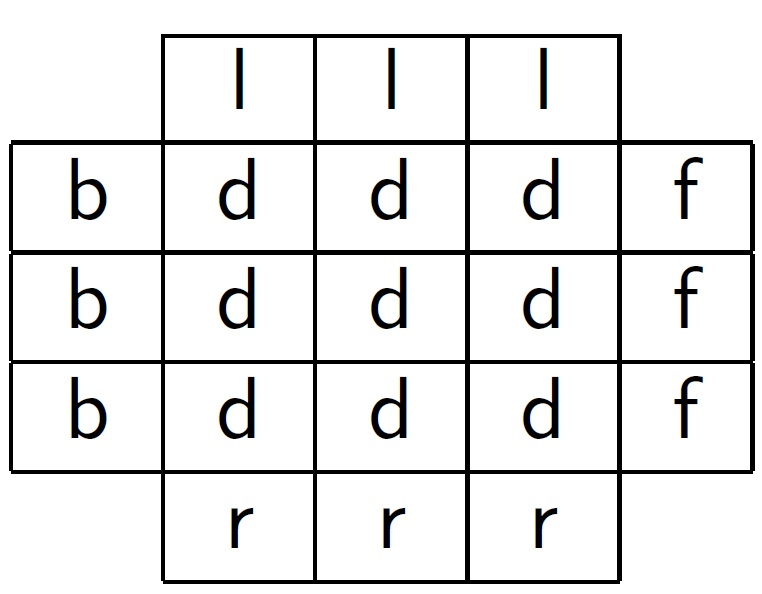
\includegraphics[scale=0.2]{input/pics/rubiks2.jpg}
		\caption{\myCaption{Remember!!}}
	\label{fig:rubiks2}
\end{figure}

So, $D(dlf) = dfr$ because the $dlf$ \cpiece{} now lives in the $dfr$ cubicle (with the down face of the \cpiece{} lying in the down
face of the cubicle, the left face of the \cpiece{} lying in the front face of the cubicle, and the front face of the \cpiece{} lying
in the right face of the cubicle). Similary, $D(dfr) = drb$, $D(drb) = dbl$, and $D(dbl) = dlf$. Do the same thing
for the edge \cpiece{}s, and then $D = (dlf dfr drb dbl)(df dr db dl)$.
